\section{Module Functions and Integration}
\label{sec:modules}
The design in Section~\ref{sec:design} is realized through three cooperating functions:
task and context assembly, shared operation dispatch, and controlled device
access with route-specific evidence. We follow one agent action through them.

\subsection{Task, Harness, and Context}
Task and chat entry points create or join a workspace channel. The task
runtime manages membership, task state, and shared execution context; a
harness registry adapts each supported agent engine to a common execution
interface. At each agent turn, the prompt builder assembles the task, active
scene description, production context, channel profile, agent binding, and
retrieved memory. This keeps engine-specific interaction behind the harness
interface while preserving the current line and operation context for the
agent.

Direct REST and selected stdio-MCP operation calls reach the same dispatcher
without a task or harness turn. REST authentication and identity resolution
follow Section~\ref{sec:executionflow}; each handler reads live route state
at invocation. Handlers receive the resolved actor, channel, and operation
arguments through the same interface for either entry route; records are keyed
by the identifiers supplied in each request. For either entry path,
prompt context and tool-catalog visibility describe available information and
capabilities, while dispatch-time checks determine write authority.

\subsection{Shared Dispatch and Device Admission}
\label{sec:governed}
The dispatcher is the shared operation boundary. It checks invocation scope
and current channel policy, then verifies the agent binding, runtime grant,
and ownership of referenced resources before selecting a handler. In the
notation of (\ref{eq:dispatch-contract}), scope and policy apply to every
call; grant is skipped only for a grant-exempt tool, and binding applies only
when references are declared. Handlers revalidate route-specific state at
execution time, using the current policy and grant for each invocation.
Scene blueprints define device and signal maps, objectives, and process
guards. Capability profiles and tool policies narrow available operations,
while bindings constrain accessible nodes, controls, and recipes. Optional
DAQ, MES, analysis, retrieval, optimization, and digital-twin services are
invoked through registered handlers. The application supplies its optimization
strategy while the framework coordinates operation execution.

Actuator writes converge on the shared DCW admission point.
For an online node write, the admissible value interval is
\begin{equation}
\mathcal{I}^{\mathrm{online}}_n(t)=
\mathcal{H}_n\cap\mathcal{B}_n\cap\mathcal{P}_n(t)\cap\mathcal{R}_n(t),
\label{eq:admission}
\end{equation}
where $\mathcal{H}_n$ is the hard engineering range and
$\mathcal{B}_n$, $\mathcal{P}_n$, and $\mathcal{R}_n$ are the baseline,
active-product, and active-recipe limits; the subscripted limits here are
distinct from the policy and binding predicates of
(\ref{eq:dispatch-contract}). Missing optional limits impose no
restriction; an empty intersection rejects the request and identifies the
excluding layer. Recipe dispatch validates the replacement recipe against
the hard, baseline, and product limits rather than the previous recipe
window. Step, interval, and hold-window checks also constrain each route.
These software checks bound commands alongside independent
programmable-logic-controller and safety-instrumented protection.

\subsection{Approval, Execution, and Evidence}
\label{sec:routes}
\label{sec:mech}
\label{sec:objective}
\label{sec:nodeexec}
\label{sec:ack}
\label{sec:agentloop}
Routes add timing and approval checks appropriate to their operation. Online
node writes enforce a 60\,s minimum spacing; recipe trials use a per-line
cadence (300\,s by default), and recipe intervals are anchored to approval.
Manual approval binds an actor and proposed operation to candidate values,
applicable limits, expiry, and the active line--product--recipe--run tuple.
After approval, the handler rechecks authority and compares the current tuple
with the approved tuple before entering DCW dispatch. Single-parameter waits
expire after 180\,s by default; recipe-dispatch approvals use a 30-minute
window. A changed recipe definition requires a new
\texttt{recipe\_apply} proposal.

Fig.~\ref{fig:hitl}(a) illustrates the four-layer value interval in
Eq.~(\ref{eq:admission}) using an illustrative rotational-speed
configuration in revolutions per minute (rpm). Panel (b)
shows a symbolic approval followed by authority and context rechecks; its
values illustrate the approval sequence.

\begin{figure*}[!t]
\centering
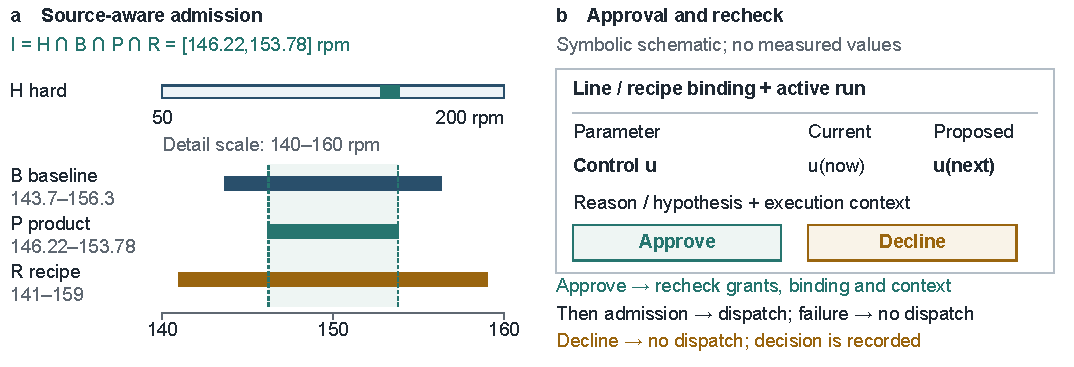
\includegraphics[width=\textwidth]{resources/fig-admission-hitl-2026.pdf}
\caption{Admission and approval boundaries. (a) An illustrative rotational-speed
configuration in revolutions per minute (rpm): online node interventions use the
four-layer interval of Eq.~(\ref{eq:admission}), whereas recipe dispatch
omits the previous recipe window. (b) Symbolic human approval binds a
proposed action and its context tuple; execution rechecks the active
line--product--recipe--run context, authority, and applicable limits before
device dispatch.}
\label{fig:hitl}
\end{figure*}

A \texttt{recipe\_trial} illustrates the operation sequence: the handler
checks the bound recipe, active run, candidate parameters, and route timing;
if required, it requests approval; after revalidation, it submits a bounded
batch through the configured driver and returns a per-parameter receipt.
The caller obtains later DAQ observations separately and may then update,
apply, or roll back a recipe. A trial neither saves nor applies a recipe
version. The driver registry maps semantic controls to configured protocol
drivers, keeping protocol details out of agent operation arguments.

Receipts and observations answer different questions. A command result is
graded as readback-verified, transport-acknowledged, or unverified; a
readback mismatch can trigger up to three reads at 2\,s intervals. Recipe
batches retain per-parameter verification outcomes. DAQ stores subsequent
timestamped process observations, while recipe versions, approvals, and
task records remain service-owned records linked where a route supplies the
corresponding identifiers. Command receipts document device execution, while
subsequent DAQ observations establish the resulting process response. This
distinction defines the evidence chain evaluated in Section~\ref{sec:eval}.

